\chapter{Vyhodnocení práce}

Výsledkem této práce je implementace systému pro porovnávání výkonu verzí softwaru
pojmenovaná PerfEval. V této kapitole bude krok za krokem ukázáno, jak se systémem pracovat.

\section{Používání systému PerfEval}

V~následujících dvou ukázkách bude vysvětleno, jak používat PerfEval. První ukázka bude
cílit na~nastínění, co~nejjednoduššího použití. Druhá část ukáže aplikaci PerfEvalu na~skutečném projektu.

\subsection{Jednoduché použití PerfEvalu}

Následující kód popisuje obvyklou posloupnost příkazů práce se systémem PerfEval.
Na začátku je nutné jej inicializovat. PerfEval bude inicializován pro použití JMHJSONParseru.
Následně se přidají výsledky měření několika (alespoň dvou) různých verzí.
Nakonec program vypíše, jestli výkonnostní testy prošly nebo ne.

\begin{lstlisting}
    #!/bin/bash
    perfeval init --benchmark-parser JMHJSONParser
    perfeval index-all-results --path tests/old_test --version old_version
    perfeval index-all-results --path tests/new_test --version new_version
    perfeval evaluate && echo "Performance test passed" | exit 0
    echo "Performance test failed" | exit 1
\end{lstlisting}

\bigskip

\subsection{Návrh skriptu pro doměření výsledků}

Následující kód nastiňuje možnost využití příkazu list-undecided. Výstupem tohoto příkazu
jsou dva tabulátorem oddělené sloupce. V prvním sloupci jsou názvy metod, pro něž systém
eviduje málo naměřených běhů. Ve druhém sloupci je uveden tento počet. Příkaz je určený
pro skriptování, proto není dodaná žádná další hlavička.

V případě, že výstupem není žádný výpis, tak je hodnot u všech testovacích metod naměřeno dostatek. Druhou alternativou
je, že v důsledku nastavení v~konfiguračním souboru systém vyhodnotil, že není možné požadovaný
počet testů doměřit. Následné vyhodnocení pak bude vyžadovat kontrolu uživatelem, protože
systém PerfEval bude vyhodnocení považovat za nevyhovující.

Skript projde všechny řádky výpisu. Pokud je výpis prázdný, tak skončí.
V~následujícím kódu je celá situace velmi zjednodušena. Nalezne se maximální počet
testů, který je zapotřebí změřit. Pro~tento maximální počet se změří výkony obou verzí znovu. Výsledky těchto měření
se zaznamenají do~systému PerfEval. Po~doběhnutí všech měření skript skončí. Vyhodnotí mezi sebou výsledky těchto
verzí a~skončí. Parametry \$1 a~\$2 jsou stará a~nová verze k~porovnání. Předpokládá se, že
příkaz measure provede měření verze zadané jako první argument a~výsledek uloží do souboru specifikovaného jako druhý argument.

\begin{lstlisting}
    #!/bin/bash

    index=1
    while true; do
        output=$(perfeval list-undecided --old-version "$1" --new-version "$2")
        if [[ -n "$output" ]]; then
            max=$(echo "$output" | cut -f2 -d$'\t' | sort -n -k | head 1)
            for ((i=1; i<=max; i++)); do
                result_file="old_version_$index"
                measure "$1" "$result_file"
                perfeval index-new-result --path "$result_file" --version "$1"

                result_file="new_version_$index"
                measure "$2" "$result_file"
                perfeval index-new-result --path "$result_file" --version "$2"
                ((index++))
            done
        else
            perfeval evaluate --old-version "$1" --new-version "$2"
            exit $?
        fi
    done

\end{lstlisting}

\subsection{Použití PerfEvalu v průběžné integraci}

Systém PerfEval je možné po vzoru unit testů používat při průběžné integraci.
V příkladu níže je uvedeno, jak může vypadat soubor \texttt{.gitlab-ci.yml} pro GitLab CI.
Uvedený vzor ilustruje, jak dodat výsledky měření do~systému PerfEval a~jak následně
spustit vyhodnocení výsledků měření dvou verzí.

Skripty \texttt{measure\_old\_version.sh} a~\texttt{measure\_new\_version.sh} v uvedeném příkladu
simulují měření výkonu, tak že přečtou výsledky z~předem připravených souborů. Tyto připravené soubory
jsou výsledky měření, které byly získány spuštěním výkonnostních testů projektu Crate \cite{crateDB}.

Výsledek porovnání je zde uložen do souboru \texttt{junit-report.xml}. Tento soubor je ve formátu JUNIT XML.
Tento formát je běžně přijímaný nástrojem Git v rámci průběžné integrace.
\bigskip
\bigskip

\begin{lstlisting}
    image: openjdk:21-jdk

    stages:
        - test

    variables:
        JUNIT_REPORT_PATH: junit-report.xml

    build:
        stage: test
        script:
            - bash measure_old_version.sh >old_measurement.json
            - bash measure_new_version.sh >new_measurement.json
            - bash perfeval.sh init --benchmark-parser JMHJSONParser
            - bash perfeval.sh index-new-result --version 1.0 --path ./old_measurement.json
            - bash perfeval.sh index-new-result --version 2.0 --path ./new_measurement.json
            - bash perfeval.sh evaluate --t-test --junit-xml-output > $JUNIT_REPORT_PATH

        artifacts:
            when: always
            paths:
            - $JUNIT_REPORT_PATH
            reports:
            junit: $JUNIT_REPORT_PATH
            expire_in: 1 week

\end{lstlisting}

\section{Nasazení systému v praxi}

V~této kapitole bude ukázáno, jak systém PerfEval funguje při~svém nasazení.
Pro ukázku byl vybrán projekt Crate \cite{crateDB}. Jedná se~o~databázový projekt
volně dostupný na platformě GitHub.

Projekt Crate byl vybrán, protože je volně dostupný, a~protože má implementované výkonnostní testy.
Tyto testy je možné spouštět samostatně přímo z~adresáře projektu a~to~i~pro~starší verze.

Systém PerfEval tedy bude použit pro porovnání vybraných commitů. Cílem tohoto
spouštění je zjistit, jestli systém PerfEval detekuje zhoršení a~případně zlepšení
výkonu.

\subsection{Výběr commitů}

Commity pro prezentování práce systému byly vybírány z~období od~21.~dubna 2020 do~11.~května 2023.
Byly vybrány ty commity, jejichž commit message obsahuje slovo „performance“ a~jejich sousední commity (pro porovnání).
Commity byly vybírány z~hlavní větve projektu. Všechny výkonnostní testy byly prováděné na~strojích stejného druhu a~konfigurace.

Z takto vybraných commitů byly dále vybrané jen ty, u~kterých bylo možné projekt bez problémů sestavit. Zároveň bylo také nutné,
aby bylo možné sestavit a~spustit výkonnostní testy. Nakonec tedy bylo vybráno a~naměřeno celkem 16 commitů z~uvedeného období.
Pro každý z~těchto commitů, který reprezentuje v~doméně systému PerfEval verzi, bylo měření provedeno celkem osmkrát.

\subsection{Výsledky porovnávání přímých sousedů}

Nástroj PerfEval byl spouštěn pro porovnání výsledků měření z~předchozí podkapitoly. Výsledky byly zaznamenány do~databáze PerfEvalu.
Ten byl předtím inicializován pro použití JMHJSONParseru. Výsledky byly zaznamenány do~databáze a~následně vyhodnocovány.
Vyhodnocování probíhalo s~použitím statistické metody bootstrap a~filtrem \texttt{--test-id}, který setřídil výsledky podle
názvů metod.

Při vyhodnocování přímých sousedů nedošlo k~zaznamenání žádného zhoršení výkonu. Přímí sousedé byly vybráni tak, že
se nalezl commit s~commit message, která obsahovala slovo „performance“ a~jejich přímý soused byl commit, který bezprostředně následoval, nebo předcházel tomuto.
Pokud by tedy PerfEval byl součástí průběžné integrace při~integrování takto vybraných commitů, tak by nebylo zaznamenáno žádné zhoršení výkonu,
a~tedy by bylo možné pokračovat v~integraci.

Ani v~jednom z~těchto případů nebylo zaznamenáno ani zlepšení výkonu na~které commit message poukazovaly.
Je tedy nutné vyřešit otázku jestli PerfEval je schopen vůbec nějaké změny výkonu detekovat.
Pro tento účel byly porovnány také bezprostředně nesousedící commity. Změny výkonu se totiž mohou kumulovat skrze více commitů.
Pokles výkonu se tedy nemusí projevit u~commitu, který změnu způsobil, ale až u~commitu, který tuto změnu dostatečně zesiluje.
Pokud by PerfEval detekoval změny na~větší vzdálenost mezi commity, tak by to znamenalo, že PerfEval je schopen detekovat změny výkonu.
Dále to znamená, že commit message uvedené u~vyhledaných commitů nereferují na~změnu výkonu provedenou v~daném commitu.

\subsection{Výsledky porovnávání nesousedících commitů}

Protože PerfEval nezaznamenal žádné zhoršení výkonu u~přímých sousedů, tak byly porovnány také přímo nesousedící commity.
Došlo tedy k~porovnání každého ze 16 commitů (vybraných v~kapitole 6.2.1) s~každým z~těchto 16 commitů, který byl novější.
Nejstarší commit byl tedy porovnán s~15 novějšími a~nejmladší commit nebyl porovnán s~žádným jiným novějším.

PerfEval porovnává pomocí příkazu \texttt{evaluate} právě dvě verze (novou a~starou).
Jako nová verze byla volena mladší ze~dvou porovnávaných verzí. Jako stará byla volena
starší ze~dvou porovnávaných verzí. Celkem tedy bylo na~16 commitech provedeno 120 takových porovnání.

Při~těchto porovnáních PerfEval ve~svém výchozím nastavení již byl schopen detekovat zhoršení výkonu.
Ačkoli všechny vybírané commity měly referovat ke zlepšením výkonu, tak PerfEval ukázal, že
u~některých výkonnostních testů došlo ke~zhoršení výkonu. Ukazuje se, že čím jsou commity
vzdálenější od~sebe ve~vývoji softwaru, tím se zvyšuje počet testů, které selhávají.
Toto pozorování je vidět na~obrázku grafu 6.1. Procentuální neúspěšnost byla spočtena jako
podíl označených zhoršení výkonu vůči celkovému počtu společných testů, které mají obě verze.

\begin{figure}
    \centering
    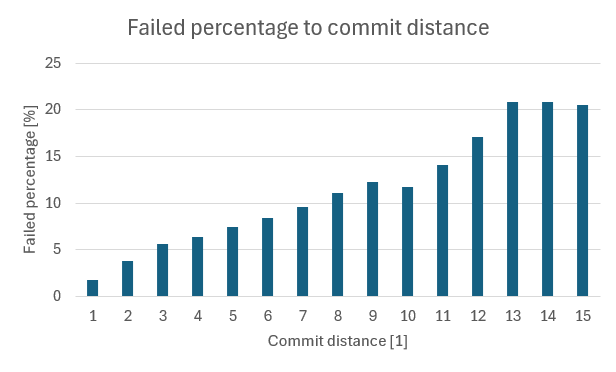
\includegraphics[width=\textwidth]{../img/failure_percentage_graph.png}
    \caption{Graf počtu testů, které selhaly, vůči vzdálenosti commitů v~čase}
\end{figure}

K~tomuto postupnému růstu poměru selhávajících testů dochází, protože se zhoršení výkonu může kumulovat skrze více commitů.
Pokud se tedy měřená metoda zhoršuje v průběhu času, tak se to projeví až u commitu, který tuto metodu dostatečně zesiluje.
Po dostatečném zesílení tohoto zhoršení se metoda zhorší natolik, že ji porovnání se~vzdálenou předchozí verzí detekuje, ačkoli
porovnání s~přímým sousedem by ji nedetekoval.

Ukazuje se tedy, že pomocí PerfEvalu je sice možné detekovat zhoršení výkonu v~rámci průběžné integrace.
Není ale vhodné jej používat jako blokující faktor při integraci. PerfEval by měl být spíše používán jako nástroj
pro detekci zhoršení výkonu v~průběhu vývoje. V~případě, že PerfEval detekuje zhoršení výkonu, tak je uživatel
schopen jednoduše zjistit, kde ke zhoršení došlo. Pokud by PerfEval byl součástí průběžné integrace jako blokující faktor,
tak by se mohlo stát, že by integrace byla zablokovaná kvůli zhoršení výkonu, který ve~skutečnosti z~větší části způsobil jiný commit.

V~grafu na obrázku 6.1 je vidět, že se zde nachází i~několik neúspěšných testů u~commitů se vzdáleností 1.
Tato porovnání byla provedena tak, že se z vybraných 16 commitů vždy vybral commit a jeho soused v tomto
výběru a ne pouze bezprostřední soused. Proto i když bylo výše uvedeno, že PerfEval nezaznamenal žádné zhoršení,
tak na grafu je vidět, že některé testy selhaly. Tato selhání byla způsobena tím, že se výkonnostní testy
se ve skutečnosti porovnávaly i~s~commity, které byly vzdáleny o~víc než jeden commit. To je způsobeno tím,
že výběr commitů byl proveden tak, že byly vybrány commity, které obsahovaly slovo „performance“ v~commit message
a~jejich sousední commity. Celý tento výběr však nejsou bezprostředně navazující commity.

Tato ukázka práce systému PerfEval netvrdí, že se výkon v~projektu Crate zhoršuje.
U~některých metod bylo zaznamenáno také zlepšení. Zlepšování výkonu softwaru totiž bývá
často něco za něco. Zlepšení výkonu jedné metody může znamenat zhoršení výkonu jiné metody.
Získané zlepšení ale může být v~některých případech tak velké, že zhoršení výkonu jiné metody
je přijatelné. PerfEval tedy může být použit jako nástroj pro detekci těchto změn výkonu,
není ale schopen v~schopen se rozhodnout zdali je změna výkonu pozitivní, nebo negativní.